\documentclass[english]{article}
\usepackage[T1]{fontenc}
\usepackage[latin9]{inputenc}
\usepackage{babel}
\usepackage{graphicx}
\usepackage{subcaption}
\usepackage[left=0.5in,right=0.5in,top=0.8in,bottom=0.5in,footskip=.25in]{geometry}
\usepackage{ocr}
\usepackage{color}
\usepackage{bm}
\usepackage{booktabs}
\usepackage{amsmath}
%\usepackage{mathabx}
\usepackage{amssymb}
\usepackage[usenames,dvipsnames]{xcolor}
\usepackage{tikz}
\usepackage{titling}
\usepackage{listings} 
\usepackage{forest}
\usepackage{caption}
\usepackage{longtable}
\usepackage{enumitem}
\usepackage{courier}
\usepackage{url}
\lstset{% 
   language=Matlab, 
   basicstyle=\small\ttfamily, 
} 
\newcommand{\ndiv}{\hspace{-4pt}\not|\hspace{2pt}}
\newcommand{\rou}[1]{\ocrfamily\small{\textbf{\textcolor{red}{#1}}}\normalfont\normalsize}
\newcommand{\var}[1]{\ocrfamily\small{\textbf{\textcolor{gray}{#1}}}\normalfont\normalsize}
\newcommand{\refline}[1]{(\protect\tikz{\protect\fill[white] (0,-0.3em) rectangle (1.8em,0.3em);\protect\draw[#1] (0,0) -- (1.8em,0);})}
\newsavebox\CBox
\def\textBF#1{\sbox\CBox{#1}\resizebox{\wd\CBox}{\ht\CBox}{\textbf{#1}}}
\title{MATH 240: Discrete Structures 1 Assignment \#5}
\author{Monorina Mukhopadhyay (ID: 260364335) Prof: E. DeCorte}
\begin{document}
\pgfkeys{/forest,
    tria/.append style={ellipse, draw},
  }
\maketitle
\section*{Problem 1}
Yes, Figure 1 shows an Eulerian graph with an even number of vertices (6) and an odd number of edges (7).
\begin{figure}[h]
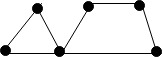
\includegraphics[width=8cm]{Q1.jpg}
\end{figure}
\section*{Problem 2}
 Let the three vertices in the centre be grouped together, and the four vertices (two on either side of the central column of vertices) be grouped together. There are more vertices in the edges (4) than in the centre(3). Any path going from one edge to another would always have to pass through the centre. Since there are more edges than centre vertices, any path that connects all the edges would have to go through the centre vertices four times, and one centre vertex would have to be visited more than once to cover all the edges.
\section*{Problem 3}
Since G is connected and bipartite, every vertex in A is connected to some vertex in B, and every vertex in B is connected to some vertex in A. 
\\ Let |A| = |B| = n. 
\\ Since the degree of each vertex in B is different, the degrees must be in the range of [1,n]
\\ Let X $\subseteq$ B. Say |X| = x where $x \leq n$ The neighbourhood of X in A is N(X), which is the set of elements in A adjacent to some element of X, and this is equal to the maximum degree of X. If there are x elements in X, the degrees of the elements must range from 1 to at least x or greater (the smallest is when the elements with degrees 1,2....,x are in X, and in this case the max. degree is x, and |N(X)| is higher for any other combination of elements in X) This means that |N(X)| $\geq$ x, and so |X| $\leq$ |N(X)|. By the Hall's theorem, there is a perfect matching in G. 
\section*{Problem 4}
Let X $\subseteq$ A be a vertex set $\implies$ |X| $\leq$ n. \\ If |X| $\leq \frac{n}{2}$ Since any vertex in X has at least degree n/2 (and therefore n/2 neighbours), the neighbourhood of X in B is at least n/2. |N(X)| $\geq \frac{n}{2}$ and therefore, |X| $\leq$ |N(X)|
\\ If |X| $\geq \frac{n}{2}$. Every vertex in B has at least n/2 neighbours in A. Since X has more than n/2 elements, some of the neighbours of each vertex in B must lie in the set X $\implies$ every vertex in B is adjacent to some elements in X $\implies$ N(X) = B. $\implies$ |N(X)| = |B| = n $\implies$ |X| $\leq n = |N(X)|$. By the Hall's Theorem, G contains a perfect matching.
\section*{Problem 5}
\begin{enumerate} [label=\alph*]
\item i.  Each vertex in A has degree d, by definition. \\ Let |A| = n. Number of edges with one end in A are d|A|.
\\ Each vertex in B also has degree d, and so number of edges with one end in B must be d|B|. 
\\ d|A| = d|B|, since the graph is bipartite (ie no edges going from A to A or B to B, so all edges with one end in A must have the other end in B.)
\\ So, |A| = |B|
\item ii.  Let X $\subseteq$ of A. Number of edges with one end in X is d|X| = k $\leq$ n = |A| = |B|.
\\ N(X) is a subset of B, since graph is bipartite and connected. So, every vertex in N(X) also has degree d. \\ Maximum number of edges with one end in N(X) is d |N(X)| since N(X) is also d regular. Since k is the number of edges going from X to N(X), $\implies$ k $\leq$ d |N(X)|. $\implies$ |X| $\leq$ |N(X)| $\implies$ G contains a perfect matching from Hall's Theorem. 
\end{enumerate}
\section*{Sources}
Compared answers and discussed solutions with Ruth Silcoff.

\end{document}